\chapter{Image Segmentation}
    \textbf{Image segmentation} is a computer vision technique that partitions a digital image into distinct regions or pixel groups, assigning labels to every pixel to simplify image analysis and understand specific objects, boundaries, or features. It separates foreground objects from the background, enabling precise identification and localization of items. \\
    While there are many ways to do Image Segmentation such as Deep Learning, Neural Networks, Convolutional Neural networks and k-means clustering. Here we are going to use Cut-based Hierarchical clustering to segment images. 

    \section{Cut-based Clustering}
        The data to be clustered is represented by an undirected adjacency graph $G$ with arc capacities assigned to reflect the similarity between the linked vertices. Clustering is achieved by removing arcs of $G$ to form mutually exclusive subgraphs such that the largest inter-subgraph maximum flow is minimized. The segmentation is achieved by effectively searching for closed contours containing isolated strong edges, while rejecting contours containing isolated strong edges. This method is able to accurately guarantee the formation of closed edge contours.
        
        For the case of an unconstrained optimal $K-$subgraph partition of $G$, the arcs selected for removal are those in a set of $K-1$ minimum cuts with the smallest $K-1$ values among all possible minimum cuts separating all pairs of vertices. The resultant clustering achieved by this method is a globally optimal solution. It minimizes the largest inter-subgraph maximum flow among all possible $K-$partitions of $G$, hence minimizing the similarity between the subgraphs (clusters). The difficulty in reaching a globally optimal solution for a particular partitional clustering technique arises from the requirement that a huge number of $K-$ partitions must be considered.

        The following Clustering Strategy can be efficiently implemented to handle graphs of size ~$2000$ vertices. In addition, this clustering technique apart from optimal $K-$subgraph partition also produces a nested sequence of partitions which are optimal for cluster numbers ranging from $2$ to $K$. \\
        The following are the steps in the clustering method:
        \begin{enumerate}
            \item {
                Construct an adjacency graph $G$ which can produce meaningful clusters.
            }
            \item {
                Construct the Gomory-Hu (equivalent min-Cut) Tree $T^*$ of $G$. 
            }
            \item {
                The optimal $K-$partition of $G$ can be equivalently obtained by simply disconnecting the $K-1$ arcs in $T^*$ with the $K-1$ smallest arc capacities.
            }
            \item {
                Each partition of nodes obtained after separating the $K-1$ minimum arcs is a resultant cluster.
            }
        \end{enumerate}
        
        \noindent However, this quickly becomes infeasible for graphs of larger size ($\geq 10^4 $ nodes) due to polynomial complexity of the algorithm.

        To overcome this problem Zhenyu Wu and Lichard Leahy present a faster hierarchical algorithm [WL93]. \\
        We are going to discuss about the algorithm in the next Section.

    \section{Hierarchical Clustering Algorithm}
        This algorithm requires construction and partition of a partially equivalent tree $T^*_c$ of greatly reduced size. This still results in an optimal solution equivalent to that obtained by partitioning the complete equivalent tree of $G$. The algorithm is based on the observation that most of the minimum cuts found in $G$ are never used since their associated cut-values are sufficiently large that the arcs in those cuts will not be removed to form subgraphs.

        \subsection{Formulation and Clustering Rationale}
            Here, it is assumed that the data set can be adequately represented by an adjacency graph $G$, where each vertex corresponds to a data point and an edge indicates a neighborhood relationship between the two linked components, and a similarity measure between these two is assigned to the arc as its flow capacity. \\
            In case of Image Segmentation one could construct such a graph in which each vertex represents a pixel in the image and edges are placed between pairs of neigbouring pixels.

            Let $G = (V,E)$ be an adjacency graph, formed from the data set with vertex $V = \{v_i,v_2,...,v_n\}$ and edge set $E = \{e_{ij}\}$ with $e_{ij}$ denoting the edge between vertices $v_i$ and $v_j$ with capacity $c_{ij}$. Here, $c_{ij}$ is a similarity measure between $v_i$ and $v_j$, i.e. the larger the edge capacity $c_{ij}$, the more similar are the vertices.

            \vspace{5mm}
            \noindent{\large \bf Theorem 6.1:} \textit{Let $G^* = (V,E^*)$ be a hypothetical complete graph with
            edge capacity $e^*_{ij} \in A^*$ equal to the maximum flow $F_{ij}$ betwen the corresponding vertices $v_i$ and $v_j$ of the original graph $G$. Then $T^*$ is flow-equivalent to the original graph $G$. Furthermore, the flow-equivalent tree $T^*$ is constructed using the Gomory-Hu algorithm is also cut-equivalent to $G$.
            }

            \vspace{5mm}
            \noindent{\large \bf Corollary 6.1 (to Theorem 6.1):} \textit{
                The $K-$partition of an undirected graph $G$, obtained by removing the $K-1$ edges with the smallest capacity in the equivalent tree $T^*$ of $G$, minimizes the largest inter-subgraph maximum flow among all possible $K-$partitions of $G$.
            }

            \vspace{5mm}
            \noindent{\large \bf Corollary 6.2 (to Theorem 6.1):} \textit{
                The $K-$partition of an undirected graph $G$, obtained by removing the $K-1$ edges with the smallest capacity in the equivalent tree $T^*$ of $G$, is unique if all K-1 edges in $T^*$ marked for removal have capacity strictly less than the remaining unmarked edges.
            }

            \vspace{3mm}
            \noindent As the number of subgraphs increases, so does the number of corresponding regions in the segmented image. Since the goal of clustering is to produce a small number of regions from the image, a stopping condition should be used to prevent for formation of too many regions. This could be achieved either interactively by terminating the edge cutting procedure when sufficient regions have been formed, or by using a threshold so that arcs with maximum flow above a given threshold are not cut. The problem os systematically choosing a suitable threshold is clearly important.

            The capacities may be any nonnegative symmetric function. In this case the following capacity function is used: \\
            \begin{center}
                $c_{ij} = k_{ij} \ \cdot \ e^{-(\frac{\mu_i - \mu_j}{\sigma})^2}$
            \end{center} 

            \noindent $k_{ij}$ denotes the number of neighboring pixels between vertices $v_i$ and $v_j$, \\
            $\mu_i$ and $\mu_j$ are the means of patches $i$ and $j$.

            \vspace{5mm}
            \noindent{\large \bf Theorem 6.2:} \textit {
                Let $G_o$ be a subgraph of an undirected graph $G$, and $F_{o,min}$ be the minimum value of the maximum flows between all pairs of vertices in $G_o$. Lets and t be an arbitrary pair of vertices in G such that the value of the maximum flow between s and t, $F_{st}$, is smaller than $F_{o,min}$. Then $F_{st}$ can be equivalently computed from the graph, $G_c$, which is obtained by condensing all vertices of $G_o$ into a single vertex.
            }

            \vspace{5mm}
            \noindent{\large \bf Corollary 6.3 (to Theorem 6.2):} \textit {
                Let $G_o$ be a subgraph of an undirected graph G. Let $F_{o,min}$ be the minimum value of the maximum flows between all pairs of vertices in $G_o$ computed using an arbitrary subgraph, $G_o$, which contains $G_o$, and let s and t be an arbitrary pair of vertices in G. If the value, $F_{st}$, of the maximum flow between s and t, computed using G, is smaller than $F_{o,min}$, then $F_{st}$ can be equivalently computed from the condensed graph $G_c$ with all vertices in $G_o$ condensed into a single vertex.
            }

            \vspace{2mm}
            \noindent The implication of Corollary 6.3 is significant since the condition under which a subgraph $G_o$, may be condensed can be checked using only a local subgraph which contains $G_o$.

            \vspace{5mm}
            \noindent{\large \bf Lemma 6.1:} \textit {
                Let $G_o$ be a subgraph of an undirected graph G, and $F^{'}_{st}$ be the value of the maximum flow between a pair of vertices, s and t, in $G_o$ computed using $G_o$. Let $F_{st}$ be the maximum flow between s and t computed using G. Then  $F{'}_{st} \leq F_{st}$.
            }

            \vspace{5mm}
            \noindent{\large \bf Theorem 6.3:} \textit {
                Let $G_o$ be a subgraph of an undirected graph G, and $F^{'}_{o,min}$ be the minimum value of the maximum flows between all pairs of vertices in $G_o$ computed in a subgraph $G^{'}_o$ which contains $G_o$. Let $G_c$ be the graph formed from G with all vertices in $G_o$ condensed into a single vertex and let $T^*_c$ is a partially cut and flow equivalent tree of G, at threshold $F^{'}_{o,min}$, in the sense that the maximum flow, $F_{st}$, and the corresponding minimum cut can be computed from $T^*_c$ for all pairs of vertices s and t in G such that $F_{st} \leq F^{'}_{o,min}$. Furthermore for all vertex pairs, s and t, in G with flow $F_{st} \geq F^{'}_{o,min}$, the maximum flow value computed in $T_c$ is also greater than or equal to $F^{'}_{o,min}$. 
            }

            \vspace{2mm}
            \noindent An \textbf{interior vertex} of a subgraph $G^{'}_o$ of $G$ is a vertex such that all of its neighbouring vertices also belong to $G^{'}_o$. A non-interior vertex is called a \textbf{boundary vertex}.

            \vspace{5mm}
            \noindent{\large \bf Theorem 6.4:} \textit {
                Let $T^{'*}_o$ be an equivalent tree of $G^{'}_o$, a subgraph of an undirected graph G, and $T^*_o$ be a branch of $T^{'*}_o$ consisting exclusively of interior vertices of $G^{'}_o$. Let $G_c$ be the graph formed from G, with all vertices in $T^*_o$ condensed into a single vertex $v^*_o$. The equivalent tree $T^*$ of G can be constructed as follows: \\
                Construct an equivalent tree $T^*_c$ for the condensed graph $G_c$, and then replace the vertex $v^*_o$ by $T^*_o$ connected at its root vertex.
            }

            \vspace{2mm}
            \noindent Here, the \textbf{root vertex} of the branch $T^*_o$ refers to the only vertex in $T^*_o$ which neighbors a boundary vertex in $T^{'*}_o$.


        \subsection{Implementation}

            \vspace{3mm}
            \noindent \textbf{Step 1)} Form the adjacency graph $G$, and then arbitrarily partition $G$ into a number of small subgraphs {$G^{'}_{0,m}$}, usually of similar size. Let $i=0$.
            
            \vspace{3mm}
            \noindent \textbf{Step 2)} For each subgraph $G^{'}_{i,m}$ find an equivalent tree $T^{'}_{i,m}$ using the Gomory-Hu algorithm.
            
            \vspace{3mm}
            \noindent \textbf{Step 3(i)} Permanently condense all the subtrees in $T^{'}_{i,m}$ which are linked by edges with capacities $\geq F_T$.
            
            \noindent \textbf{Step 3(ii)} Temporarily condense all the maximal interior branches of this resulting tree to form a condensed subgraph $G^{'}_{i,m,c}$.
            
            \vspace{3mm}
            \noindent \textbf{Step 4)}  If there is only one subgraph in {$G^{'}_{i,m,c}$}, then denote the resulting equivalent tree as $T^{'*}_c$ and go to Step 6. \\
            Otherwise continue to Step 5.
            
            \vspace{3mm}
            \noindent \textbf{Step 5)} Group {$G^{'}_{i,m,c}$} into subsets, each containing a number of neigbouring subgraphs of {$G^{'}_{i,m,c}$}. By connecting the subgraphs in each subset using the inter-subgraph edges, we form a new subgraph set ${G^{'}_{i+1,m}}$. Let $i = i+1$, and go to Step 2.
            
            \vspace{3mm}
            \noindent \textbf{Step 6)} Expand back all the temporarily condensed vertices in $T^{'*}_c$ to construct the partially equivalent tree $T^*_c$ of the original graph $G$.
            
            \vspace{3mm}
            \noindent \textbf{Step 7)} Remove successively edges in $T^*_c$ in order of increasing edge capacity until a given stopping condition is met. A clustering constraint may also be attached in this last step.

            \vspace{5mm}
            \noindent Since constructing an equivalent tree for graphs with few vertices is very fast, it is usually more efficient to start the algorithm with a large number of very small subgraphs. The only restriction in selecting the threshold $F_T$ is that no minimum cut with value larger than $F_T$ may be used for partitioning the graph $G$. Ideally the threshold $F_T$ should be chosen as the value of the largest minimum cut which will be made in partitioning $G$ so that the clustering is most efficient.


        \section{Results and Improvements}
        In this section I am going to discuss and show the results of the final Segmented Image on different categories of Image as generated by the above mentioned Algorithm. Furthermore, I am going to provide some of my own improvements to the above algorithm (keeping the core algorithm same) to achieve a better Runtime and also to improve the final Clustered images, to produce better results. \\
        The methods discussed above (in the paper [WL93]) were for Black-and-White images having a single parameter (intensity) describing each image. \\
        Here, I extended this to support RGB images having 3 parameters per pixel by using edge capacity function (between 2 pixels sharing an edge) as:-
        \begin{center}
            $c_{ij} = e^{-(\frac{\sum_{k=1}^{C}(\mu^k_i - \mu^k_j)^2}{C \ \cdot \ \sigma^2})}$
        \end{center}
        where C is the number of Channels (parameters per pixel).

        \vspace{7mm}
        \noindent \textbf{1. Synthetic Images (generated using MS Paint)}
        \begin{figure}[H]
            \centering
            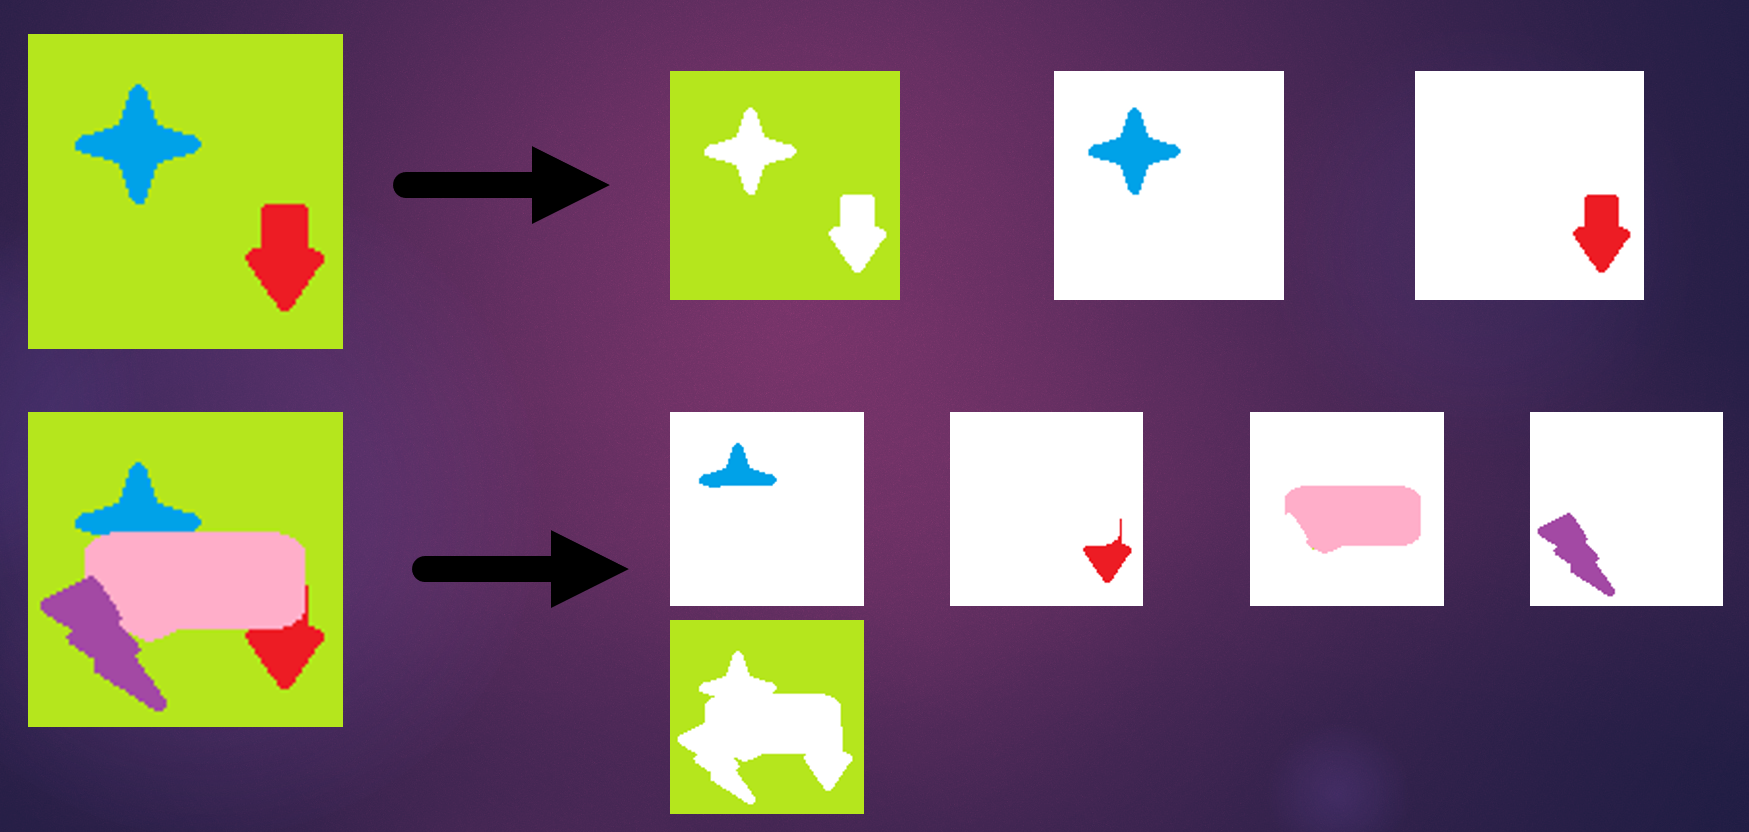
\includegraphics[width=1\linewidth]{figures/Synthetic_image.png}
            \caption{Synthetic Image}
            \label{fig:placeholder}
        \end{figure}

        \noindent We observe that \textbf{Synthetic Images} are separated very well by the Algorithm without any further modifications or improvements to it. All the elements in the image are properly segmented including the background.

        \clearpage
        \noindent \textbf{2. Real Images (high colour gradient)}
        \begin{figure}[H]
            \centering
            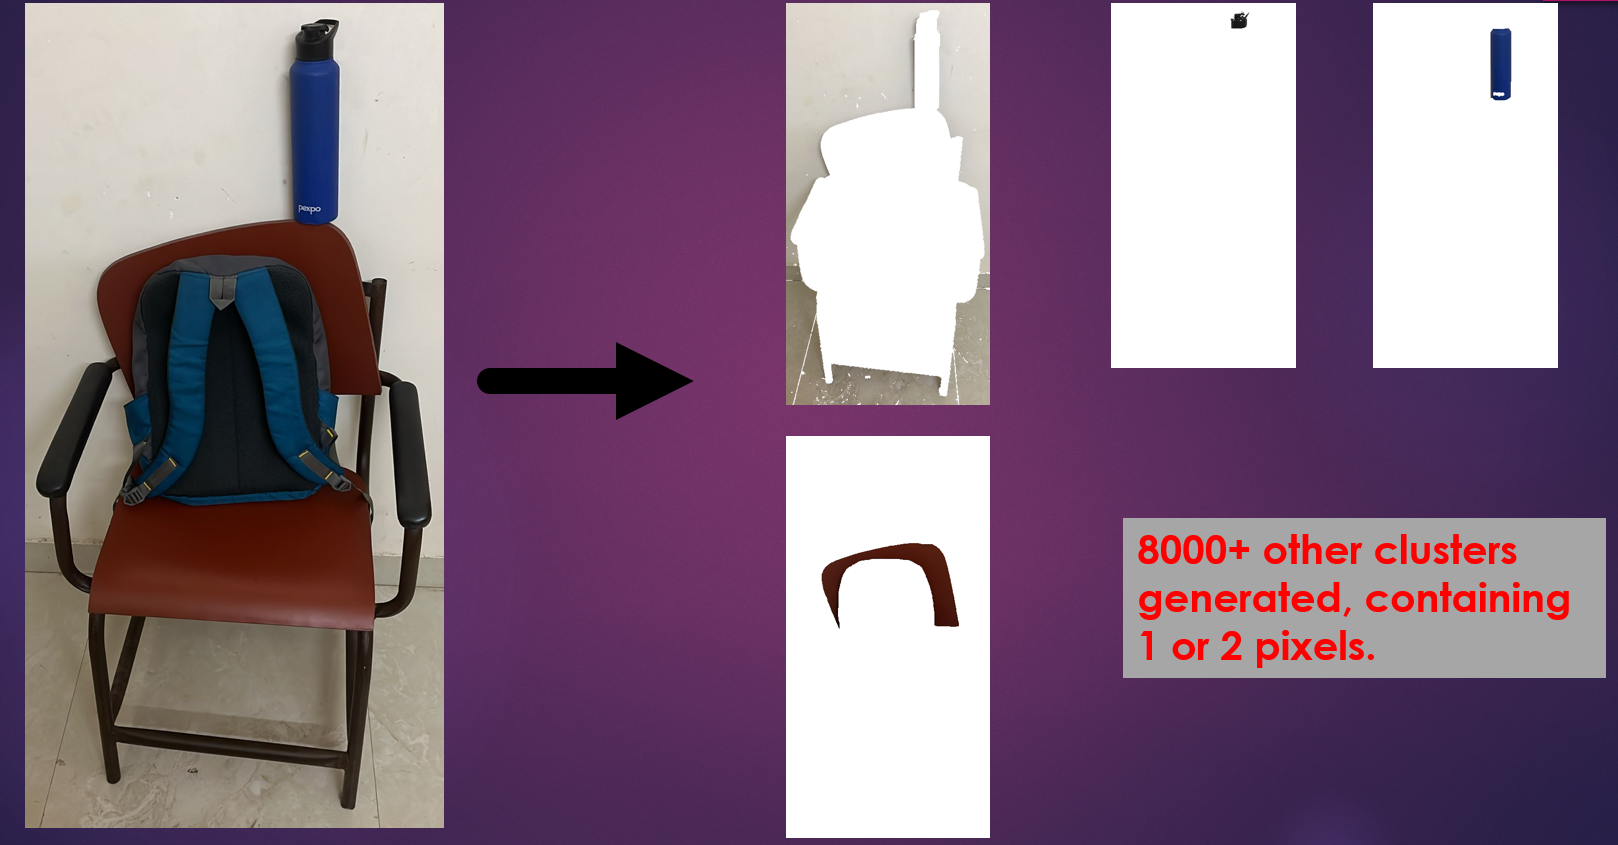
\includegraphics[width=1\linewidth]{figures/Real_Image_1.png}
            \caption{Real Images (having high colour gradient)}
            \label{fig:placeholder}
        \end{figure}

        \noindent In case of a \textbf{Real Image} even though the background separation and other components seem to be properly separated, there are more than 8000 clusters generated from this Image, which is not the Segmentation that we want to achieve.

        \vspace{3mm}
        \noindent \textbf{Reason:} The primary reason behind this is the Algorithm separates first the easily \indent \indent \indent \indent \indent separable clusters. \\
        Consider the the case where there is a very small black speck present in a white background. Now, we don't want to separate that part of image since that is just some error/variance in the image which we would like to ignore. However, since black and white generate the highest contrast and as a result the edge capacities between then will be very low and also a very low min-Cut value. This results in separation of that speck and is treated as a separate cluster.

        \vspace{5mm}
        \noindent \textbf{Improvement-1: } Setting lower limit on the the number of nodes/pixels that should be \indent \indent \indent \indent \indent \indent \indent \indent \indent present in a cluster. \\
        This is ensured by a merge step after the initial partition, where for each cluster having $\leq MIN\_SIZE$ nodes/pixels in a cluster is merged to another cluster which bears the highest similarity (max. min-Cut) to the current cluster.

        \begin{figure}[H]
            \centering
            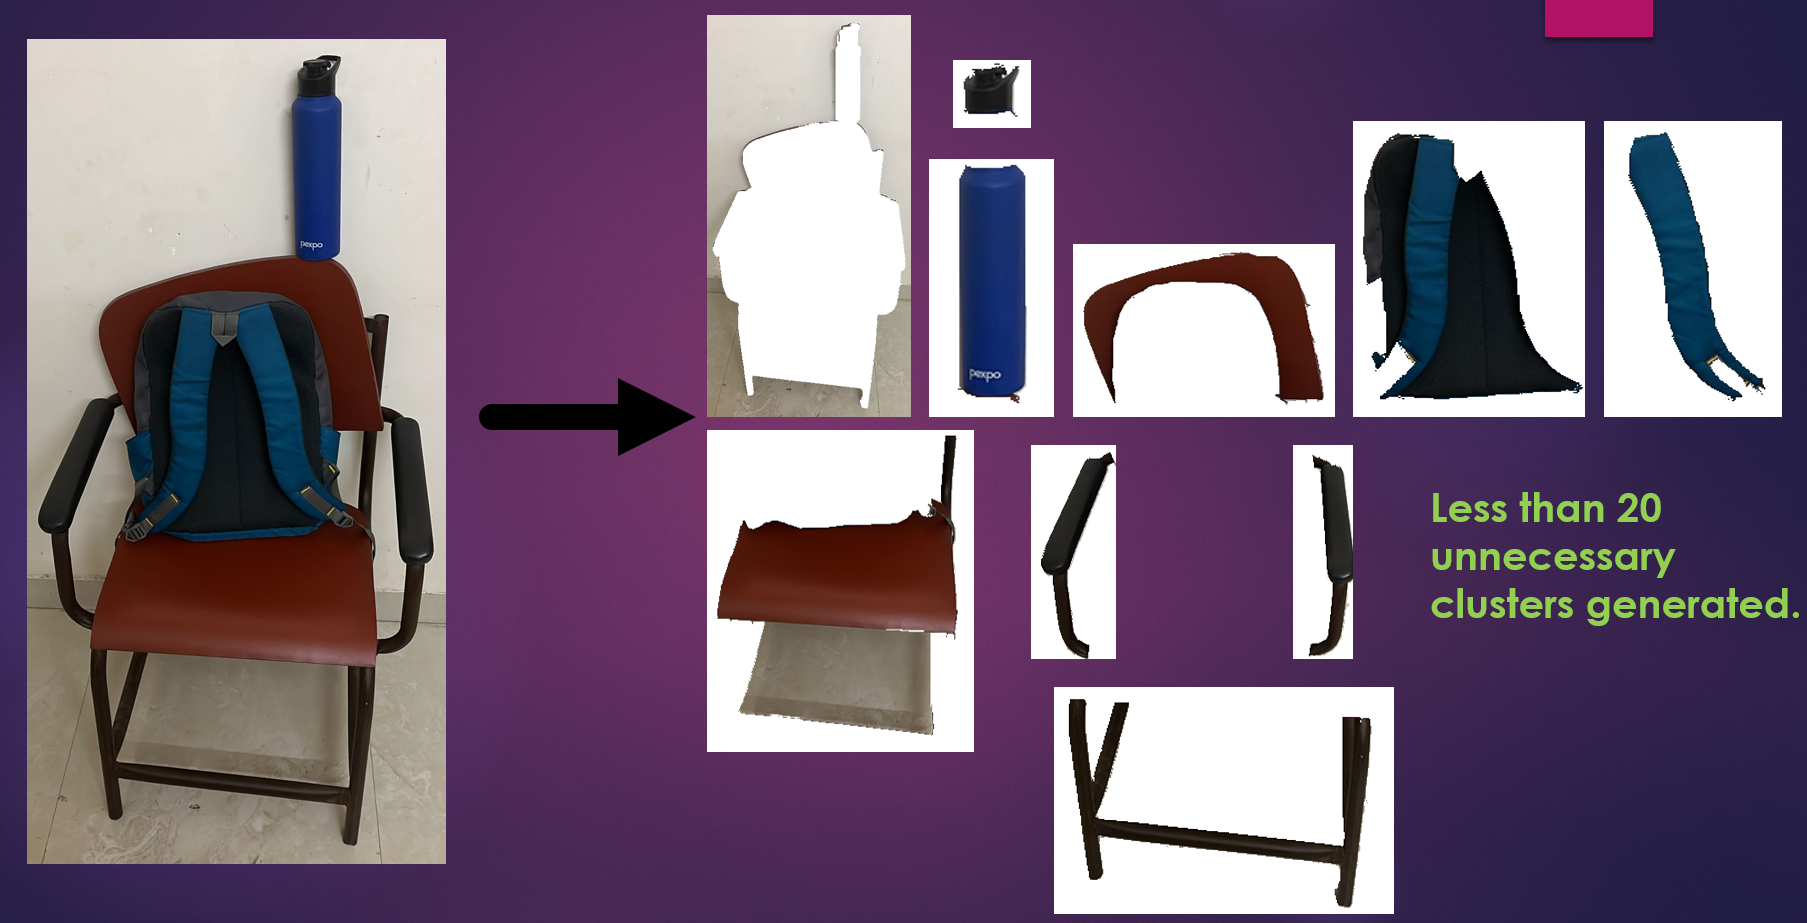
\includegraphics[width=1\linewidth]{figures/Real_Image_after_Improvement_1.png}
            \caption{Real Image (after Improvement-1)}
            \label{fig:placeholder}
        \end{figure}

        \vspace{2mm}
        \noindent Here we observe that after implementing Improvement-1 for minimum Cluster size all the major elements for the Image are now properly separated. Furthermore, there are only less than 20 other clusters apart from the main ones (containing physical elements) which appear to be useless compared to the 8000+ clusters from previous case.

        \vspace{7mm}
        \noindent \textbf{3. Natural Images}
        \begin{figure}[H]
            \centering
            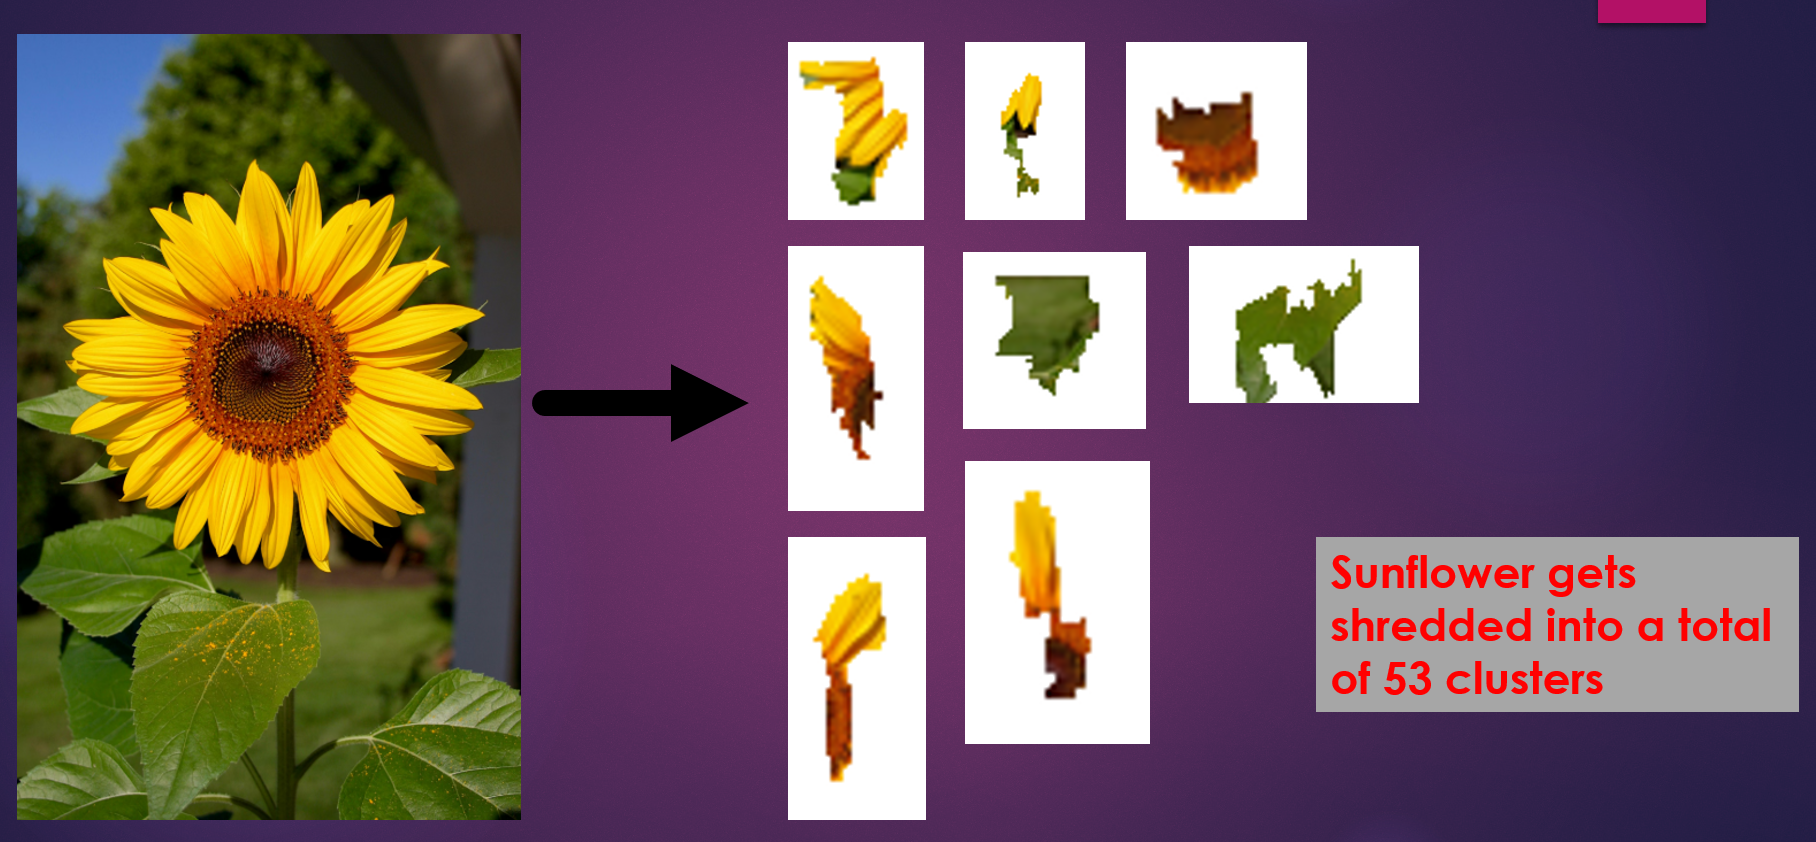
\includegraphics[width=1\linewidth]{figures/Natural_Image_1.png}
            \caption{Natural Image - 1}
            \label{fig:placeholder}
        \end{figure}

        \vspace{2mm}
        \noindent In case of this Natural Image containing a sunflower with some background in it, we see that the Sunflower gets shredded into multiple different parts and the parts(clusters) of it also don't have any meaningful physical interpretation.

        \vspace{3mm}
        \noindent \textbf{Reason:} Most likely the reason behind this is that the pixels don't have enough contextual information to perform the clustering. Taking only adjacent pixels as edges in case of Natural Images is not enough context to perform the clustering.

        \vspace{5mm}
        \noindent \textbf{Improvement-2: } Instead of only taking Orthogonal adjacent pixels as edges, increase the Neighborhood size to 3 or 5 pixels surrounding it and also optionally adding diagonal edges to add more surrounding context for the current pixel. \\ 
        Even though this Improvement results in better overall clustering it also affects the execution time for Clustering since increasing neighbourhood also means increasing the number of edges in the graph.

        \begin{figure}[H]
            \centering
            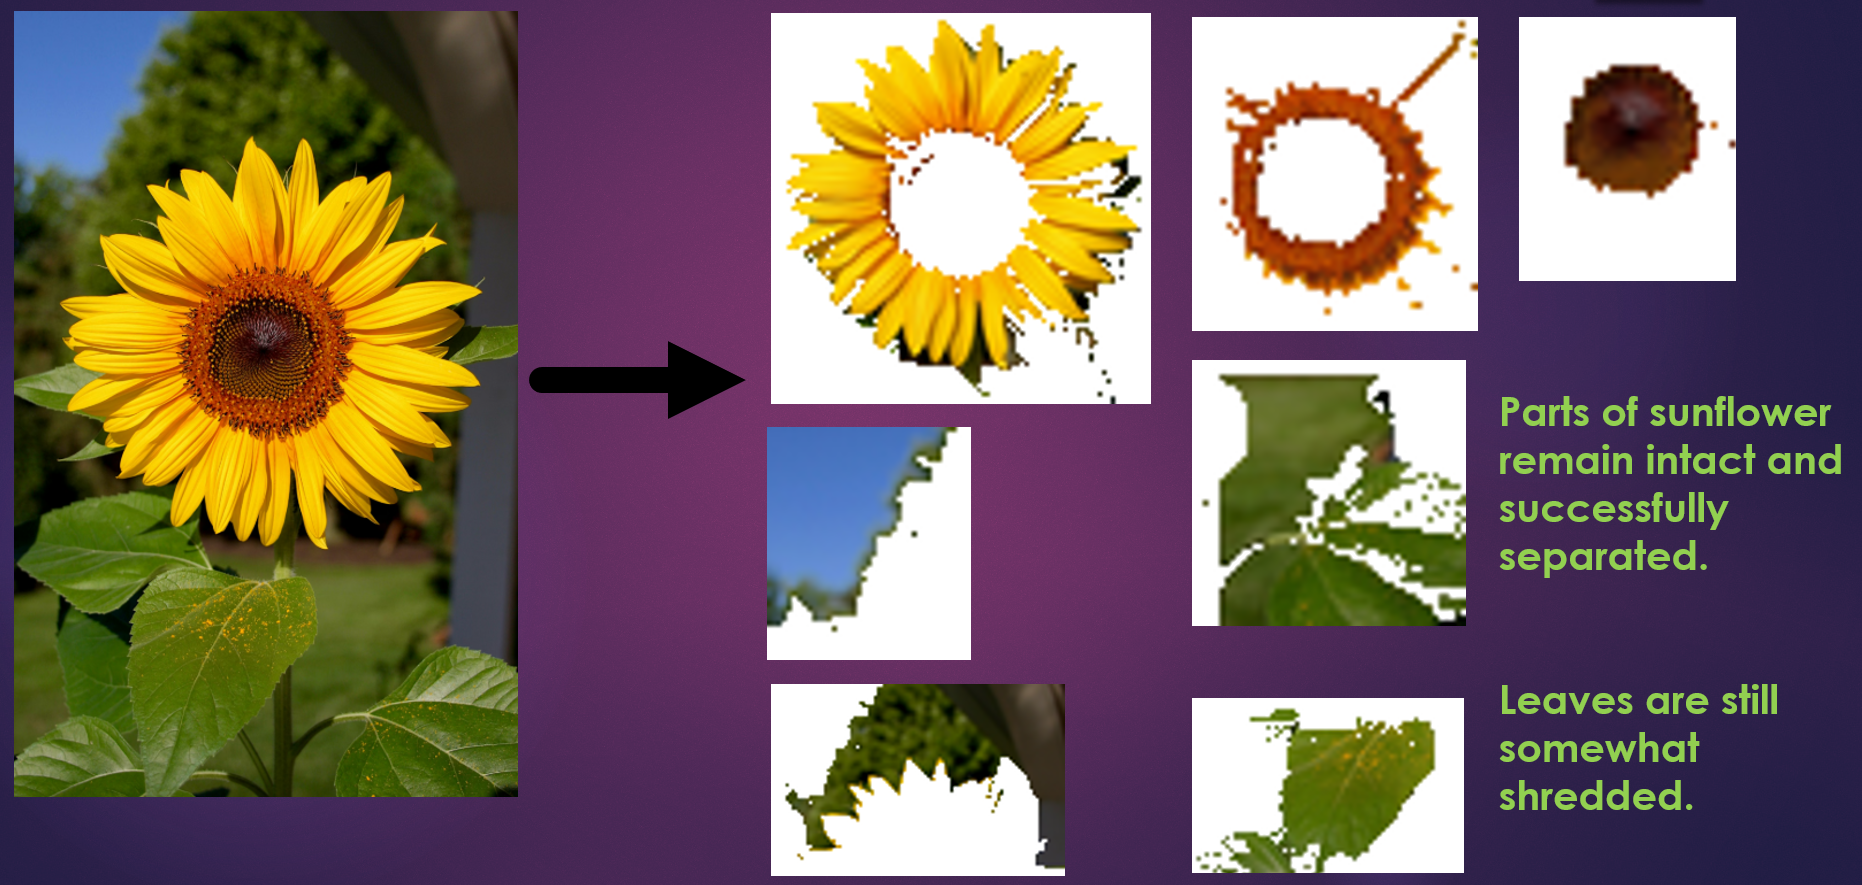
\includegraphics[width=1\linewidth]{figures/Natural_Image_1_after_Improvement2.png}
            \caption{Natural Image - 1 (after Improvement-2)}
            \label{fig:placeholder}
        \end{figure}

        \vspace{2mm}
        \noindent After Implementing Improvement-2, now we see that Segmentation is much better. Sunflower instead of getting shredded into pieces is now divided into 3 parts (Outer part having Yellow petals, Middle Orange Ring and the Inner Brown Core part). The background sky and other parts are also somewhat separated. \\
        Leaves are better clustered although the leaves are still somewhat shredded. This is because of poor/low colour gradient i.e. Green Leaves in a Green Background.

        \clearpage
        \subsection{Execution Time Improvements}
            Till now we have discussed improvements for better resultant Clustering. \\
            Here, I am going to provide a few methods to optimize the overall Execution Time required to generate the final Clusters from the Initial Input Image.

            \begin{enumerate}
                \item {
                    \textbf{Parallelizing Local Subgraph Computation:} Observe that Step 2 (from SubSection 6.2.2 - Implementation) - computing Gomory-Hu Tree for each local subgraph is independent for each of the local subgraphs $G^{'}_{i,m}$. \\ 
                    Here, we can divide the computation of different $T^{'}_{i,m}$ into different threads i.e. for a given Hierarchy Level $i$ we can parallelize over the values of $m$.
                }
                \item{
                    \textbf{Mathematically finding Optimal Hierarchy Depth:} Instead of going for Higher levels of hierarchy and subgraph merging until the no. of subgraphs becomes 1 (Step 4 - first case), we can stop at an earlier Level if we observe that there are very few Node or Edge condensations in the graph. Unnecessarily going for higher levels of Hierarchy without significant Node/Edge condensations just leads extra computation time. This in-turn results in a worse overall computation time than the trivial Cut-based Clustering approach as discussed earlier. \\
                    Consider the analogy in the case of FFT (Fast-Fourier Transform) where we stop at a base case if the two vectors to be multiplied have sizes less than a certain value and compute that case using the Trivial Brute Force Multiplication Approach.                    
                }
                \item{
                    \textbf{Maintaining Bipartiteness after each Condensation Step:} Since the initial graph generated from the Image is a lattice graph and is therefore Bipartite, we can attempt to preserve this Bipartiteness property of the Graph throughout the Clustering process. This helps because when computing the Gomory-Hu Tree and we are doing $n-1$ flow computations. In case of Bipartite graphs Worst Case flow computation time = $O(E\sqrt{V})$. Also, since the graphs generated from images are sparse graphs i.e. $E = O(V)$, we have overall worst case Gomory-Hu Tree construction time:-    $O((V-1)\ \cdot \ E\sqrt{V}) = O(V \ \cdot \ V\sqrt{V}) = O(V^2\sqrt{V})$. \\
                    However, there are 2 issues with this:
                    \begin{itemize}
                        \item {
                            Since, we are trying to maintain bipartiteness at each Step, number of Edge Condensation will always be = 0. \\
                            Because, if two adjacent nodes sharing an edge are condensed into a single node then bipartiteness property will be broken. Also, since the Condensations are constrained, this also results in lower Node condesations. So overall, this method even though has better worst case time might lead to worse overall execution time due to lower Node/Edge Condensations.
                        }
                        \item {
                            Dinic's algorithm which is used for Flow computation here already has very low flow computation time on average. So, improvement in asymptotics might not be a very high improvement over Dinic's average case complexity. Even though it has a worst case time of $O(V^2E)$, for most cases it works below $O(V^2)$ overshadowing any significant improvement in computation times.
                        }
                    \end{itemize}
                }
            \end{enumerate}

        \subsection{Other Improvements}
            Apart from \textbf{Improvement-1} and \textbf{Improvement-2} presented previously, here I provide some other possible additional improvements which might lead to better Final Clustering.

            \begin{enumerate}
                \item {
                    \textbf{Optimally choosing Hyperparameters based on the input image rather than Hardcoding:} There are several Hyperparameters present in the Implementation such as - \textit{WINDOW\_SIZE, THRESHOLD, MIN\_CLUSTER\_SIZE, NEIGHBOURHOOD}. Instead of fixing those values as compile-time we can find an optimal configuration of these Hyperparameters based on the Input Image, since different Images have different requirements. \\
                    E.g- A higher Resolution image will most likely need a higher MIN\_CLUSTER\_SIZE compared to a lower one. \\
                    Choosing THRESHOLD based on the color gradients of the Image and then choosing the edge value at say the $10^{th}$ percentile.
                }
                \item {
                    \textbf{Processing input separately for R,G,B Channels and then combining them:} Instead of generating an edge capacity based on the difference between R,G,B intensities of 2 pixels and summing then up we can divide the image into 3 parts and then construct separate clusterings for the 3 parts. Finally, using some heuristic we can combine all those clusterings to generate a final clustering. \\
                    This is further enchanced by the fact that the core algorithm for this clustering was built for single Channel (greyscale) images. Dividing up the image effectively ensures each individual Channel is a greyscale (single parameter per pixel) image.
                }
                \item {
                    \textbf{Capacity function based on the type of Image:} We are using the same capacity function for all types of Images irrespective of their final goals. \\
                    Instead of that we can choose different capacity functions based on the type of Image (Greyscale, Synthetic, Real or other Natural Image) and the final aim of Clustering to potentially further improve the clusters.
                }
            \end{enumerate}


    \section{Advantages}
        Major advantages to the above mentioned Clustering technique primarily are:-
        \begin{enumerate}
            \item {
                \textbf{Unsupervised:} Unlike ML models, no previous training data or labelled dataset is needed for clustering the Images.
            }
            \item {
                Since, Learning is Unsupervised there is no training time required for previous computations. We can directly process Images without any previous inputs.   
            }
            \item {
                If the Image has large potions of similar coloured regions, there will be high Node/Edge condensations. In those cases, overall execution time will be very low due to extremely reduced size of final condensed graph.
            }
        \end{enumerate}

    \section{Drawbacks}
        Along with the above discussed Advantages, this Hierarchical Clustering method also has some serious (major) Drawbacks and Disadvantages some of which are tied intricately to the functioning of the core algorithm.

        \begin{enumerate}
            \item {
                \textbf{Poor results in case of Natural Images:} This method of clustering basically relies on high contrast between colours in neighbouring pixels for Segmentation/Clustering. Natural Images generally tend to have a low colour gradient. In those cases it becomes especially hard to segment out various parts of the Image.
                \begin{figure}[H]
                    \centering
                    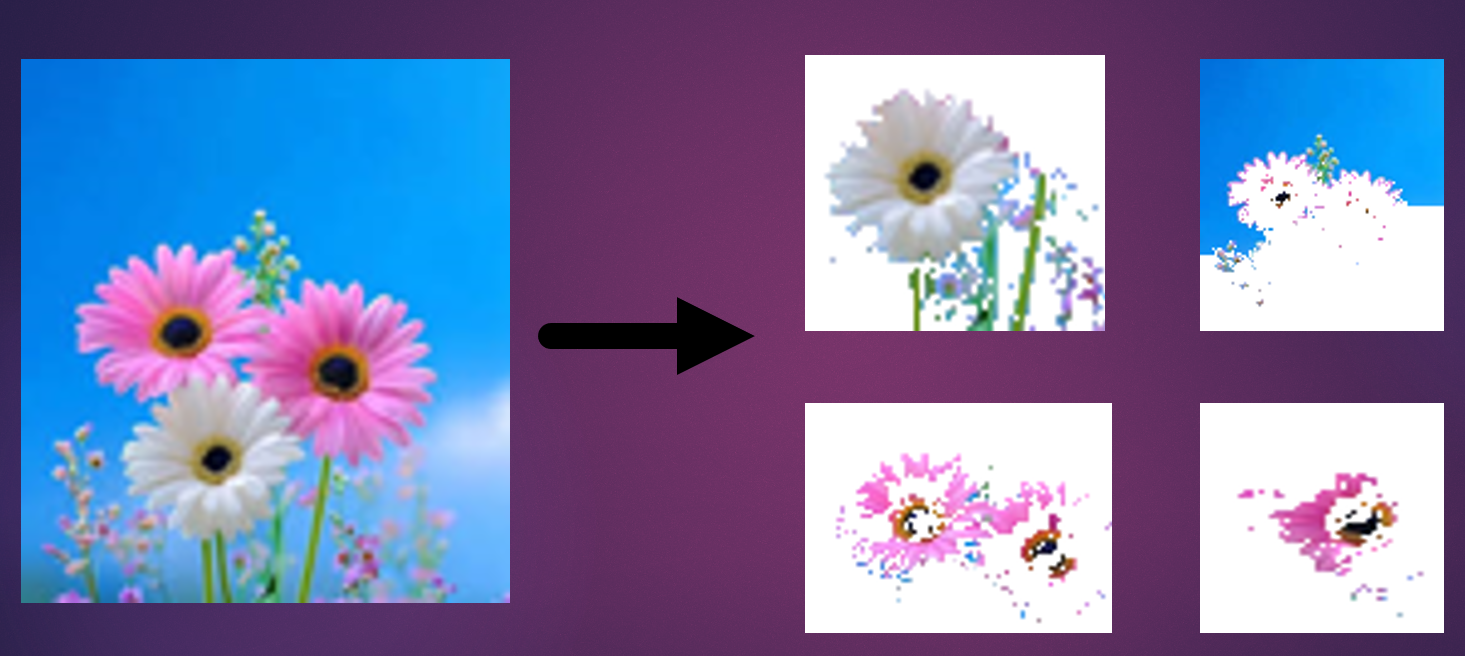
\includegraphics[width=1\linewidth]{figures/Natural_Image_2.png}
                    \caption{Natural Image - 2 (Somewhat unsuccessful Segmentation)}
                    \label{fig:placeholder}
                \end{figure}
                We can see that among the 3 flowers in the image only the White one having the highest contrast was properly Segmented along with the background Sky. It completely failed as segmenting the other 2 flowers with low Contrast.
            }
            \item {
                For higher resolution images such as 1k, 2k or 4k the number of nodes in the graph is very high (multi-millions) and as a result the execution time is also very high.
            }
            \item {
                \textbf{Lack of Context (Over-Segmentation):} A single object having different colours in different regions will be segmented into various parts (clusters), since the primary objective of this algorithm is to "Cluster on the basis of Colour". \\
                However, this might not be the expected result in most real-life scenarios as we generally want to keep the object as a whole and separate one object from another, rather than "One colour from Another". \\
                In that case we need more context signifying that the parts of a single object are related to one another and should be kept within a single cluster. This however, relates more to (and is solved by) ML-based Clustering, and is a fundamental drawback of Cut-based Image Segmentation algorithms.
            }
        \end{enumerate}